\section{Implemenation Details and Demonstration}
\label{sec:impl}
We implement both a backend program, a server program and a frontend program for our project.  The backend consists of a data training program and data transferring program. We build our data training program by Python, which is composed of two parts. The first part is a data training algorithm that provides data that used for network generation. This data training algorithm will output a certain sentence with a underlined word, several alternative words and network data that encapsulated as JSON data.  The network data include server networks the frequency that the word co-occurs with other words in the training corpus. The server is made of Flask, which is a microframework for Python. The server takes the output of backend program as input, and transfer the data to front end when the front end asks. At last but not least, the front end is the part with the function of user interface and data visualization. It asks the server to get the data generated by the backend.  We develop the main function of front end by Javascript. The relationship of the three parts is shown in Figure 5. 

\begin{figure}[h]
\centering
		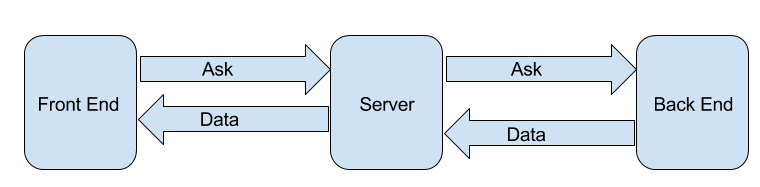
\includegraphics[width=\linewidth]{figure/workflow}
	\caption{workflow of Interactive Word Network Visualization}
	\label{fig:frp_demo}
\end{figure}

As is shown in Figure 5, the browser request the data of sentence, words, and network when the web page is loaded; then the server pass this request to the backend; the backend response with related data and the server pass it to the front end. 
The front end will request data with special parameter when the user chose some words and click submit button. Then the server pass the request to the backend. The backend will push some data new that related with the parameter. The server aslo pass this data. At last, the front end will show new networks related with the user's last choice.
\subsection{Javascript}

\subsection{Flask}

Flask is a microframework for Python. The "micro" in microframe work means Flask aims to keep the core simple but extensible.

\begin{figure}[h]
\centering
		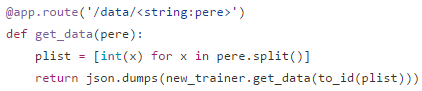
\includegraphics[width=\linewidth]{figure/FlaskHttp}
	\caption{Flask HTTP Method}
	\label{fig:flshttp}
\end{figure}
As is shown in Figure 10, the server will run this part of code when it receive a HTTP GET request with route Host/data/$\langle$para$\rangle$, where $\langle$para$\rangle$ is used as parameter that can be passed by the function "get$\_$data()", which is a function work with backend and return the data gotten from backend.

\begin{figure}[h]
\centering
		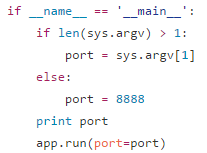
\includegraphics[width=\linewidth]{figure/FlaskRun}
	\caption{Flask run server}
	\label{fig:flsrun}
\end{figure}

The Figure 11 shows how flask run a server on a certain port. As is show, the function "app.run(port)" runs the program as a server on the port.